\documentclass[12pt]{article}

\usepackage[margin=1in]{geometry}
\usepackage{amsmath,amsthm,amssymb}
\usepackage{graphicx}
\graphicspath{ {./images/} }

\newcommand{\N}{\mathbb{N}}
\newcommand{\Z}{\mathbb{Z}}

\newenvironment{theorem}[2][Theorem]{\begin{trivlist}
\item[\hskip \labelsep {\bfseries #1}\hskip \labelsep {\bfseries #2.}]}{\end{trivlist}}
\newenvironment{lemma}[2][Lemma]{\begin{trivlist}
\item[\hskip \labelsep {\bfseries #1}\hskip \labelsep {\bfseries #2.}]}{\end{trivlist}}
\newenvironment{exercise}[2][Exercise]{\begin{trivlist}
\item[\hskip \labelsep {\bfseries #1}\hskip \labelsep {\bfseries #2.}]}{\end{trivlist}}
\newenvironment{reflection}[2][Reflection]{\begin{trivlist}
\item[\hskip \labelsep {\bfseries #1}\hskip \labelsep {\bfseries #2.}]}{\end{trivlist}}
\newenvironment{proposition}[2][Proposition]{\begin{trivlist}
\item[\hskip \labelsep {\bfseries #1}\hskip \labelsep {\bfseries #2.}]}{\end{trivlist}}
\newenvironment{corollary}[2][Corollary]{\begin{trivlist}
\item[\hskip \labelsep {\bfseries #1}\hskip \labelsep {\bfseries #2.}]}{\end{trivlist}}

\begin{document}

Consider the following graphical model:

\begin{figure}[h]
\centering
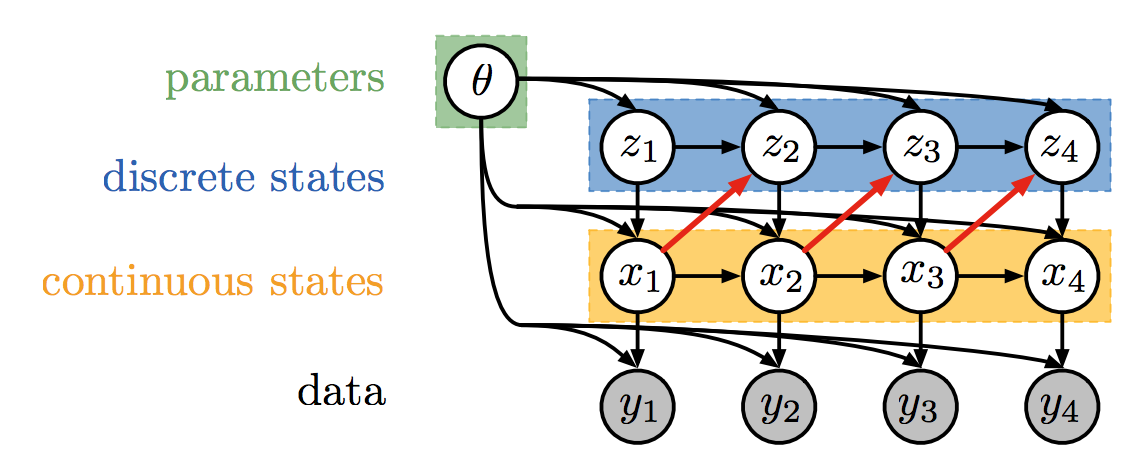
\includegraphics[width=8cm]{graphical}
\caption{Recurrent Switching Dynamic System}
\label{mode}
\end{figure}

where $\vec{z}$ is a categorical latent variable, $\vec{x}$ is a gaussian latent variable, and $\vec{y}$ are bernoulli observed variables. We wish to derive a lower bound on $\log p(\vec{y})$ for variational inference.

\begin{align}
    \log p(\vec{y}) &\geq \int_{\vec{z}} \int_{\vec{x}} q(\vec{z},\vec{x}|\vec{y}) \log \frac{p(\vec{y},\vec{x},\vec{z})}{q(\vec{z},\vec{x}|\vec{y})} d\vec{x} d\vec{z} \\
                    &= \int_{\vec{z}} \int_{\vec{x}} q(\vec{z}|\vec{x})q(\vec{x}|\vec{y}) \log \frac{p(\vec{y}|\vec{x})p(\vec{x}|\vec{z})p(\vec{z})}{q(\vec{z}|\vec{x})q(\vec{x}|\vec{y})} d\vec{x} d\vec{z} \\
                    &\approx \sum_{\vec{z}} \sum_{\vec{x}} \log \frac{p(\vec{y}|\vec{x})p(\vec{x}|\vec{z})p(\vec{z})}{q(\vec{z}|\vec{x})q(\vec{x}|\vec{y})}
\end{align}
where $\vec{x} \sim q(\vec{x}|\vec{y})$, $\vec{z} \sim q(\vec{z}|\vec{x})$. Critically, we do not extract out a term $KL[\cdot]$ since there will be no closed form for a product of a categorical and gaussian variable.

From Fig.~\ref{mode}, we can extract the following factorizations:

\begin{align}
    p(\vec{y}|\vec{x}) &= \prod_{t=1}^{T} p(y_t|x_t) \\
    p(\vec{x}|\vec{z}) &= \prod_{t=1}^{T} p(x_t|z_t) \\
    p(\vec{z}) &= p(z_1)\prod_{t=2}^{T} p(z_t|z_{t-1},x_{t-1}) \\
    q(\vec{x}|\vec{y}) &= q(x_1|\vec{y})\prod_{t=2}^{T} q(x_t|x_{t-1},\vec{y}) \\
    q(\vec{z}|\vec{x}_1, ..., \vec{x}_K) &= q(z_1|\vec{x}_1, ..., \vec{x}_K)\prod_{t=2}^{T} q(z_t|z_{t-1},\vec{x}_1, ..., \vec{x}_K)
\end{align}
where $T$ is the sequence length, and $K$ is the domain of $\vec{z}$ (number of categories) i.e. there are $K$ number of possible dynamical systems. To infer the next $z_t$, we need to know all of them. So we can write the evidence lower bound as:

\begin{align}
    \sum_{z_1,...,z_T} \sum_{x_1,...x_T}[& \sum_{t=1}^T(\log p(y_t|x_t) + \log p(x_t|z_t)) \\
    & + \sum_{t=2}^T (\log p(z_t|z_{t-1},x_{t-1}) - \log q(x_t|x_{t-1},\vec{y}) - \log q(z_t|z_{t-1},\vec{x}_1, ..., \vec{x}_K)) \\
    & + (\log p(z_1) - \log q(x_1|\vec{y}) - \log q(z_1|\vec{x}_1, ..., \vec{x}_K))]
\end{align}
where $x_1 \sim q(x_1|\vec{y})$, $x_t \sim q(x_t|x_{t-1},\vec{y})$, $z_1 \sim q(z_1|\vec{x}_1, ..., \vec{x}_K)$, $q_t \sim q(z_t|z_{t-1},\vec{x}_1, ..., \vec{x}_K)$, each of which are parameterized by an RNN (or $K$ RNNs) in reverse order. To optimize this, we use the Gumble-softmax relaxation of $\vec{z}$.

\end{document}